\chapter{Implementation}
\label{chap3}

\section{Triangulation of regular implicit srufaces}
\label{triangulation-implicit}

In this section, we shortly describe the algorithm for triangulation of the regular
parts of implicit surfaces introduced in bachelor's thesis \cite{korecova2021triangulation}.

The algorithm creates triangles iteratively, one at a time. The new triangle is
created at the edge of the existing triangle. The new point is projected on the
surface using the well-known iterative Newton-Rhapson method, the 
fast-converging method for root finding of a function $y=f(x)$. The condition 
for convergence of this method is to provide a point on the function sufficiently
close to the root. We use this method to find the root of the implicit
function lying on the line, which is in the direction of the gradient of the implicit
function. This approach is displayed in the Figure~\ref{img:29}.
\begin{figure}
    \centerline{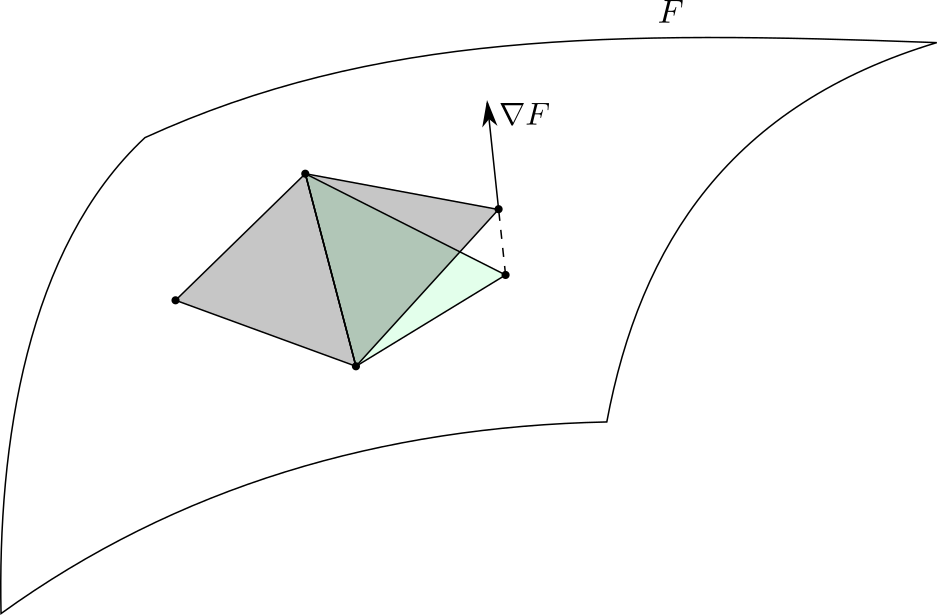
\includegraphics[scale=0.5]{images/img29}}
    \caption[Projecting the point on the surface]
    {Projecting the point on the surface in the direction of the gradient.}
    %id obrazku, pomocou ktoreho sa budeme na obrazok odvolavat
    \label{img:29}
\end{figure}

After the new point is projected on the surface, conditions are checked. 
Some of these conditions are based on the Delaunay triangulation introduced
by Hilton \cite{hilton1996marching}. The Delaunay condition checks
if some other points are in the proximity of the circumcenter of the new triangle.
The conditions minimize the chances of a triangle intersection.
If the new triangle intersects with some existing triangles, the algorithm
tries to connect the new triangle to the existing points of the mesh in its proximity.

The algorithm is enriched with the possibility to triangulate adaptively
to the curvature of the surface using the approach presented by Akkouche 
\cite{akkouche2001adaptive}. It can also triangulate surfaces in the
bounded volume - axis-aligned bounding box, given by six numbers - minimal
and maximal value for each of the three coordinate axes.

The algorithm was implemented using brute force. The queue of the edges
on the mesh border $-$ \textit{active edges}, was being iteratively updated. 
In each step, an edge from the active edges queue was removed, and the creation of a new triangle near this edge was attempted.
If the new triangle was successfully created, the edge has become 
\textit{inside edge}, in case of failure, the edge has become 
\textit{checked edge}. The last characterization of an edge is for
the edges with both end-points lying on the bounding box, these edges
are called \textit{bounding edges}.

As a part of our work, we reimplement the algorithm to be more effective by
using advanced data structures, such as the half-edge data structure 
\cite{kettner1999using} and the range tree \cite{lueker1978data}.

\section{Data structures for triangulation algorithm}
\label{sub2.5}

\subsection{Half-edge data structure}
Triangular mesh is given by vertices, non-oriented edges and triangular faces.
There are multiple methods for mesh representation. The straightforward one -
list of vertices, edges and vertices does not provide any information about
the local surroundings of the vertices, edges and faces and, therefore, the searching
for incident faces or incident edges is complicated and inefficient.

In 1975, Baumgart \cite{baumgart1975polyhedron} presented a representation
using winged edges, which was further improved in 1985 by Weiler \cite{weiler1985edge}
who presented the modification called a half-edge data structure.
Both of these representations are edge-based representations, each edge stores
references (pointers) to the surrounding vertices, edges and faces. One can easily extract information about the
surrounding vertices, edges and faces.

In the half-edge representation, edges are split into two halves of directed edges.
Each half-edge
stores reference to its initial vertex, left face, opposite half-edge and left
traverse - predecessing and succeeding half-edge. A visualization of the
half-edge is displayed in the Figure~\ref{img:32}. An example of half-edge
representation is shown on the Figure~\ref{img:31} and 
tables~\ref{tab:5},~\ref{tab:6},~\ref{tab:7}.

\begin{figure}
    \centerline{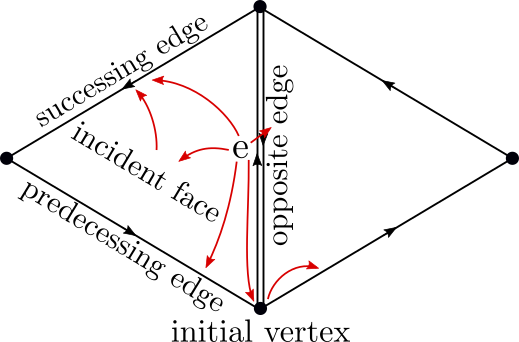
\includegraphics[scale=0.5]{images/img32}}
    \caption[Visualisation of the half-edge data structure]
    {Visualization of the half-edge data structure.}
    %id obrazku, pomocou ktoreho sa budeme na obrazok odvolavat
    \label{img:32}
\end{figure}

\begin{figure}
    \centerline{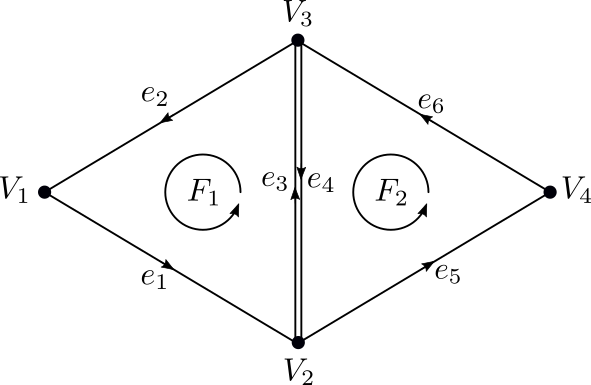
\includegraphics[scale=0.5]{images/img31}}
    \caption[Example of half-edge representation]
    {Example of half-edge representation.}
    %id obrazku, pomocou ktoreho sa budeme na obrazok odvolavat
    \label{img:31}
\end{figure}

\begin{table}[]\centering
    \begin{tabular}{|c|c|c|ccc|}
    \hline
    \hline
    Edge  & Vertex       & Face        & \multicolumn{3}{c|}{Edges}                            \\ \hline
          & Initial      & Incident    & Predecessor            & Successor          & Opposite         \\ \hline\hline
    $e_1$ & $V_1$        & $F_1$       & $e_2$            & $e_3$           &                  \\ \hline
    $e_2$ & $V_3$        & $F_1$       & $e_3$            & $e_1$           &                  \\ \hline
    $e_3$ & $V_2$        & $F_1$       & $e_1$            & $e_2$           & $e_4$            \\ \hline
    $e_4$ & $V_3$        & $F_2$       & $e_6$            & $e_5$           & $e_3$            \\ \hline
    $e_5$ & $V_2$        & $F_2$       & $e_4$            & $e_6$           &                  \\ \hline
    $e_6$ & $V_4$        & $F_2$       & $e_5$            & $e_4$           &                  \\ \hline\hline
    
    \end{tabular}
\caption{Edge table of a half-edge data structure for the Figure~\ref{img:31}.}
\label{tab:5}
\end{table}

\begin{table}[]
    \centering
    \begin{tabular}{|c|ccc|c|}
    \hline
    \hline
    Vertex  & \multicolumn{3}{c|}{Coordinates}          & Edge            \\ \hline
          & x            & y            & z           & Outgoing edge   \\ \hline\hline
    $V_1$ & $x_1$        & $y_1$        & $z_1$       & $e_1$           \\ \hline
    $V_2$ & $x_2$        & $y_2$        & $z_2$       & $e_3$           \\ \hline
    $V_3$ & $x_3$        & $y_3$        & $z_3$       & $e_2$           \\ \hline
    $V_4$ & $x_4$        & $y_4$        & $z_4$       & $e_6$           \\ \hline\hline
    \end{tabular}
\caption{Vertex table of a half-edge data structure for the Figure~\ref{img:31}.}
\label{tab:6}
\end{table}

\begin{table}[]
    \centering
    \begin{tabular}{|c|c|}
    \hline
    \hline
    Face  & Edge            \\ \hline\hline
    $F_1$ & $e_1$           \\ \hline
    $F_2$ & $e_4$           \\ \hline\hline
    \end{tabular}
\caption{Face table of a half-edge data structure for the Figure~\ref{img:31}.}
\label{tab:7}
\end{table}

The half-edge data structure is implemented in a way which does not provide 
neighborhood information for non-manifold meshes.
As our algorithm creates non-manifold meshes, we implement the half-edge data
structure with the modification $-$ each point has references to all outgoing edges
instead of just one outgoing edge. 

\subsection{Range tree}
The range tree is a tree data structure used for geometric search.
The range tree holds a list of points and answers queries about
the points in the given range. When used in three-dimensional space, 
the range corresponds to the three-dimensional interval.
The advantage of the range tree compared to other tree structures for 
three-dimensional search, such as a quad-tree or k-d tree, is a fast query
time. The implementation we used \cite{rangetree} answers the query for 
the set of points in a given three-dimensional
interval in $\mathcal{O}(log^3n+k)$, where $n$ is the number of
the points in the tree, and $k$ is the number of points in the three-dimensional
interval.

\subsection{Mesh structure}
The triangular mesh consists of vertices, edges and faces. We use the half-edge 
data structure for mesh representation and the range tree for the time-efficient search of points in three-dimensional intervals.
The mesh structure used for maintaining and modifying the triangular mesh
consists of:
\begin{itemize}
    \setlength\itemsep{-2mm}
    \item list of vertices,
    \item list of half-edges,
    \item list of faces,
    \item range tree of all vertices.
\end{itemize}
Vertex consists of 
\begin{itemize}
    \setlength\itemsep{-2mm}
    \item three coordinates,
    \item index of itself in the list of vertices,
    \item list of indices to all outgoing edges.
\end{itemize}
Half-edge consists of 
\begin{itemize}
    \setlength\itemsep{-2mm}
    \item six coordinates,
    \item index of itself in the list of half-edges,
    \item index of the initial vertex in the list of vertices, 
    \item index of the terminal vertex in the list of vertices,
    \item index of the opposite edge in the list of half-edges,
    \item index of the predecessing edge in the list of half-edges,
    \item index of the succeeding edge in the list of half-edges,
    \item index of the incident face in the list of faces,
    \item boolean values stating if the half-edge is active, checked, 
    bounding or inside.
\end{itemize}
Face consists of
\begin{itemize}
    \setlength\itemsep{-2mm}
    \item nine coordinates,
    \item index of incident half-edge in the list of half-edges.
\end{itemize}

\subsection{Algorithm runtime}
During the algorithm, new points, edges and triangles are added in
at the end of the respective list in the mesh. 
The algorithm is implemented as a single pass through the list of 
mesh edges. 
If the edge is classified as active, the algorithm proceeds 
to attempt to create the triangle near the edge. 
The triangle is being created the same way as in the brute-force
algorithm.
With this approach, we do not need to
maintain the queue of active edges. As the new edges are added at 
the end of the list, it behaves as a queue.

When checking for the conditions for the newly created triangle, the 
proximity within the mesh provided by the half-edge data structure is
insufficient. Here, the range tree is used. To find the triangles in the
proximity of a point $P$, all mesh points in a three-dimensional interval
around this points are found using the range tree. The triangles are then 
extracted by finding the incident faces of outgoing edges of the points
found by the range tree.

\textbf{Time complexity of the algorithm:}
The number of edges, points and triangles in the mesh is asymptotically 
equal. Let us denote the number $n$. The query time for the three-dimensional 
range tree is $\mathcal{O}(log^3n+k)$, where $k$ is the number of points
reported by a given query. In each step of the algorithm, a constant number of
operations and a constant number of queries to the range tree is performed.
Therefore, the overall time complexity of producing the mesh with $\mathcal{O}(n)$
faces is $\mathcal{O}(n (log^3n+k))$